\documentclass[../thesis.tex]{subfiles}
\begin{document}
\chapter{Simulation Structure Change}
\label{ch:pruning}
The work in this section involves both re-writing existing functions for more general usage and redesigning the structure of the system to further support improvements made on the model side. As illustrated earlier, model part of the system is now declared through x-macros and thus, it was necessary to redesign simulation sections to connect to and optimize changes made on means of model representation. In addition, to support a special biological mode, the old simulation section as well as numerical methods have minimal configurability and reusability. To address this problem, I intend to design new classes and functions to reimplement the \textit{Euler's Method} integration, and added modularity so that the new system is no longer model specific, but instead can be re-applied to or easily updated based on other biological models. 
\section{Methodology}
For further isolation of reactions and other simulation process, a new \textit{context} class is created. In a biological system, it provides a scope for various simulations, and in \textit{segmentation clock network}, each instance of \textit{context} class is equivalent to a cell. There is a unique identifier inside \textit{context} class and it is used as the second template parameter for functions in $model\_impl.hpp$ shown earlier. \\
\\
Placed inside simulation, the \textit{context} is essentially a wrapper class inside simulation that interacts with reactions. It encapsulates function implementation and is responsible for calculating rate change and updating concentration levels. It also provides necessary information for calculation and updating concentration levels, including step size and time step. With such functions and a unique identifier, the system can easily iterate through all \textit{context} instances and perform designated tasks with enough information from both simulation and model. \\
\\
 Updating active rates of each reaction is the first step of simulation process. Active rate describes the rates of change at one particular time step for all reactions and is equivalent to the notion of derivative in a differential equation. To update the active rates, functions are designed to cooperate well with \textit{x-macros} used during model declaration; in particular, function is placed inside a for loop over all reactions and is able to automatically generate lines of code to invoke functions for calculating rates for each of the reactions. An example of how \textit{x-macros} works in the system in is shown in \textit{context} implementation file (Figure \ref{fig:step1}). The code is written according to \textit{x-macros}. Earlier the system iterates through each \textit{context} instance to invoke member functions and now the system iterates through all \textit{reaction\_ids} and invoker each member function for that reaction. Thus two template parameters together provide easy access to all combinations of member functions and reactions. As shown in Figure \ref{fig:step1pre}, the preprocessor is able to automatically generate specific code based on the \textit{context} and the \textit{reaction\_id}. Along with model separation, new simulation mechanism allows high level of flexibility. 
 \begin{figure}[h]
\centering
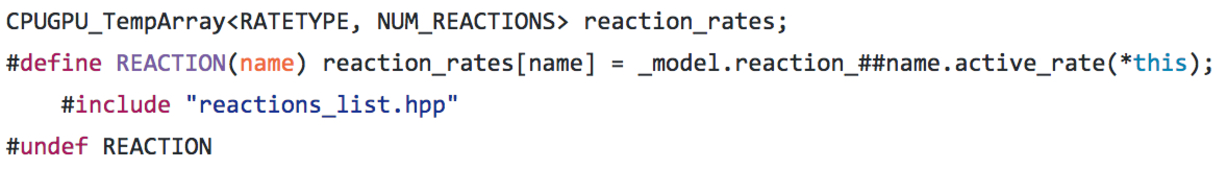
\includegraphics[width=0.9\textwidth]{step1}
\caption{Function for Updating Reaction Rates}
\label{fig:step1}
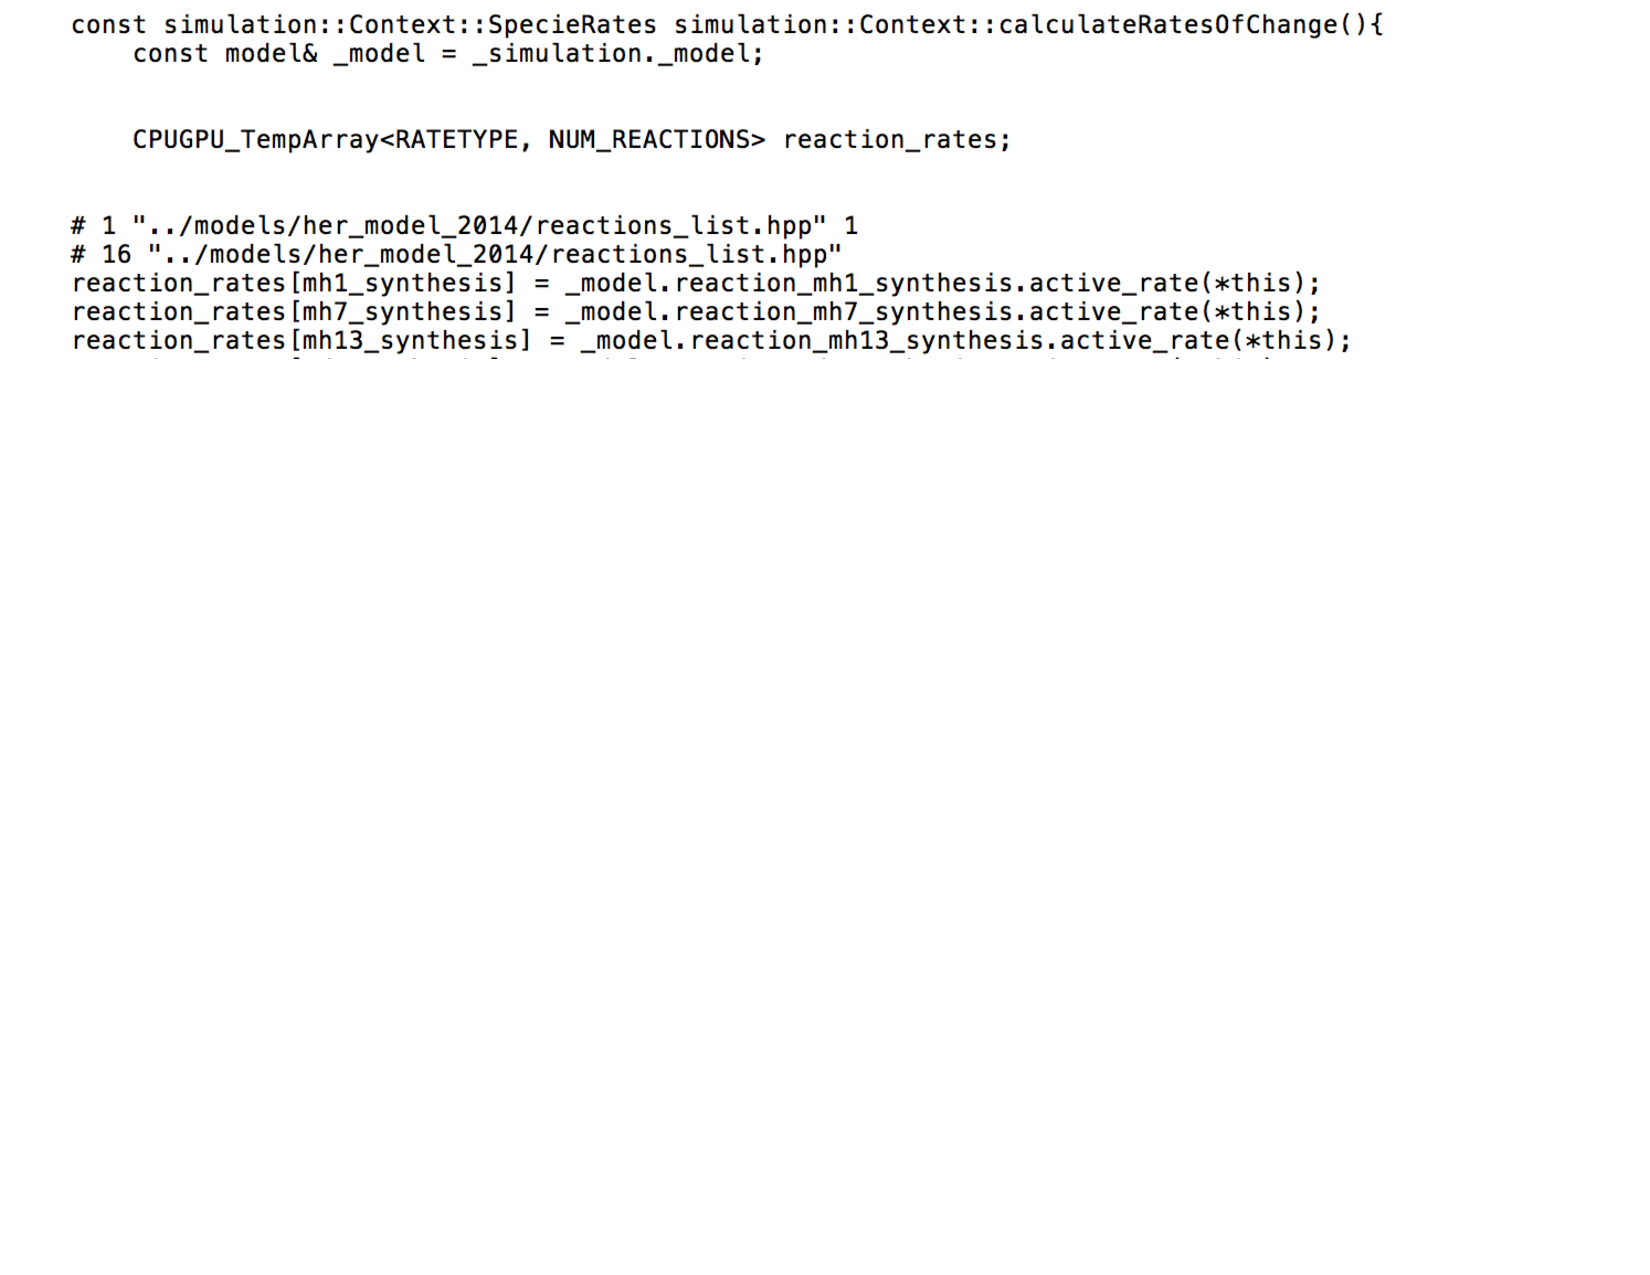
\includegraphics[width=1.0\textwidth]{step1pre}
\caption{Function for Updating Reaction Rates After Preprocessing}
\label{fig:step1pre}
\end{figure}

 \textit{X-macros} provide a foundation for the reusability of the simulation section as it ensures that the template function is configured to run with any biological models as long as model information is input under specified restrictions.\\
\\
The second step of simulation is to apply numerical methods to predict concentration levels of all species at the next time step and this is where active rates at current time step is necessary along with concentration level of each species. The new system also implements a simple \textit{Euler's Method} as its numerical solver. In the new system, I first aggregate all reactions as well as their influences on each of the species through \textit{x-macros}  (Figure \ref{fig:step1}, \ref{fig:step2}) and then apply them collectively along with concentration level of current step to estimate the concentration level of next time step (Figure \ref{fig:euler}). Through those methods applied, two subsections of updating concentration level is entirely separated from each other, which will then render much high level of freedom in either part.

 \begin{figure}[h]
\centering
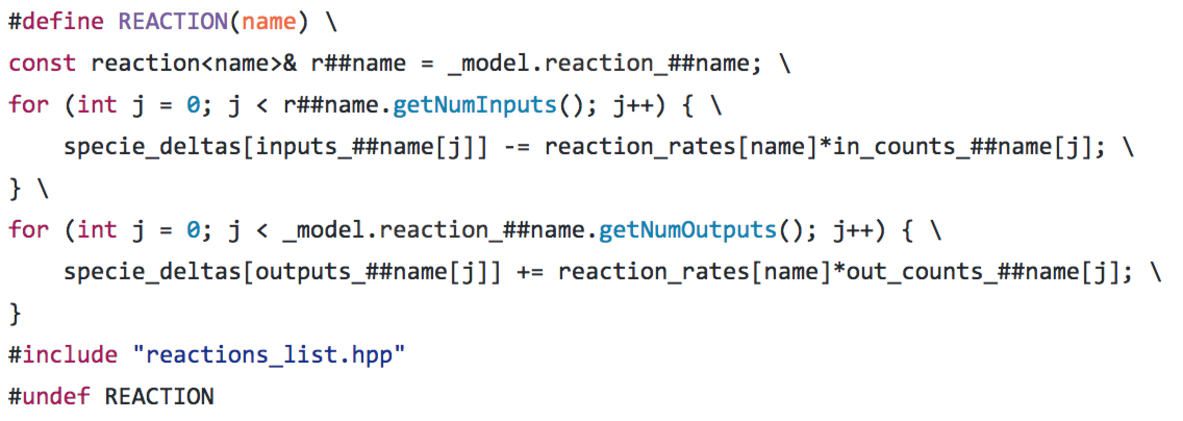
\includegraphics[width=0.9\textwidth]{step2}
\caption{Function for Collecting Derivatives at a Time Step}
\label{fig:step2}
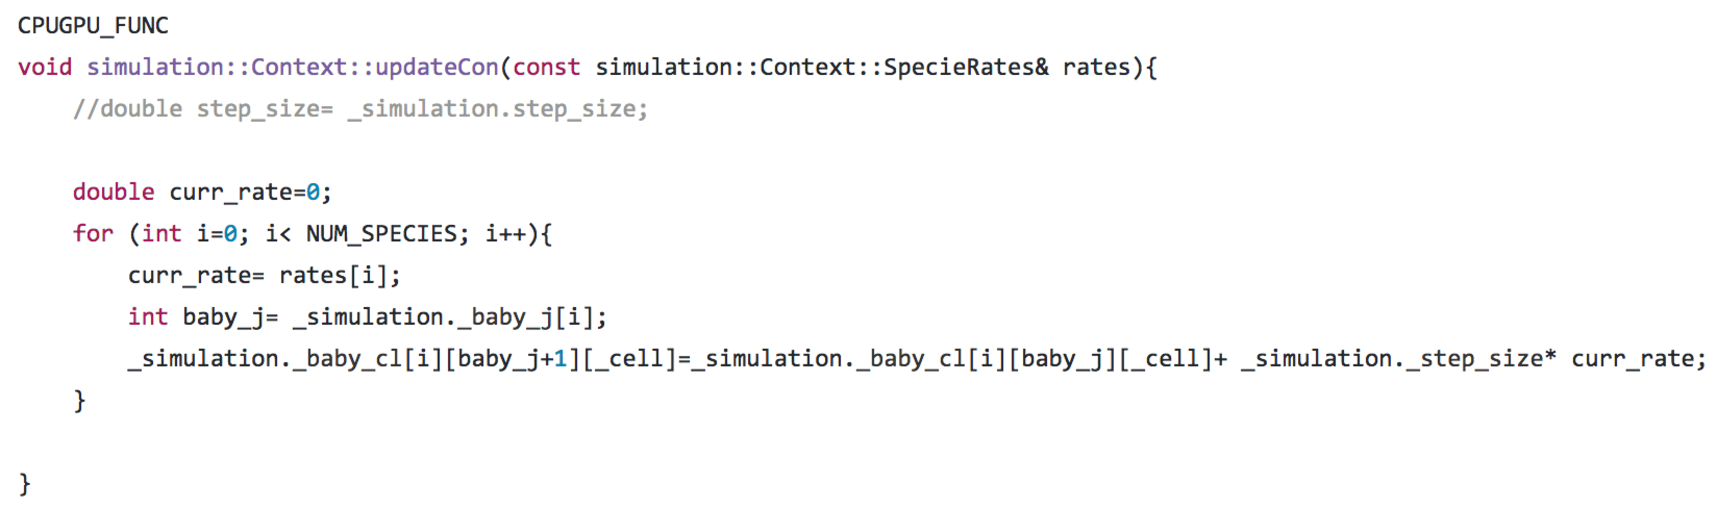
\includegraphics[width=0.9\textwidth]{euler}
\caption{Implementation of \textit{Euler's Method}}
\label{fig:euler}
\end{figure}

\section{Results}
Results for usage of \textit{x-macros} is clearly illustrated above. This is extraordinarily helpful because iteration through species or reactions takes place across the entire system and now the system is capable of generating code based on the model input.\\
\\
Updating active rates and concentration level were integrated in form of differential equations in the original system and each reaction may be calculated multiple times since it may contribute to concentration level changes of various species. Below is one of the thirteen differential equations in the original system (Figure \ref{fig:step3}) along with its corresponding implementation of this equation (Figure \ref{fig:oldeuler}). All model information is hard coded into the implementation of \textit{Euler's Method} and almost all differential equations are implemented separatedly in the original system. Thus, to change the numerical solver, the methodology applied to update concentration levels, of the original system was extremely complicated and time comsuimg. \\
\\
With the changes made in the new system, \textit{Euler's Method} is implemented in one place and could be applied for all reactions. Therefore, if a new numerical solver, such as \textit{Runge-Kutta Method},  is used, implementation of this solver will take place inside just one function and can be applied to all reactions with no further adjustments except storing more past concentration levels and active rates (for example \textit{Runge-Kutta Method} requires concentration levels from multiple time steps). 
 \begin{figure}[h]
\centering
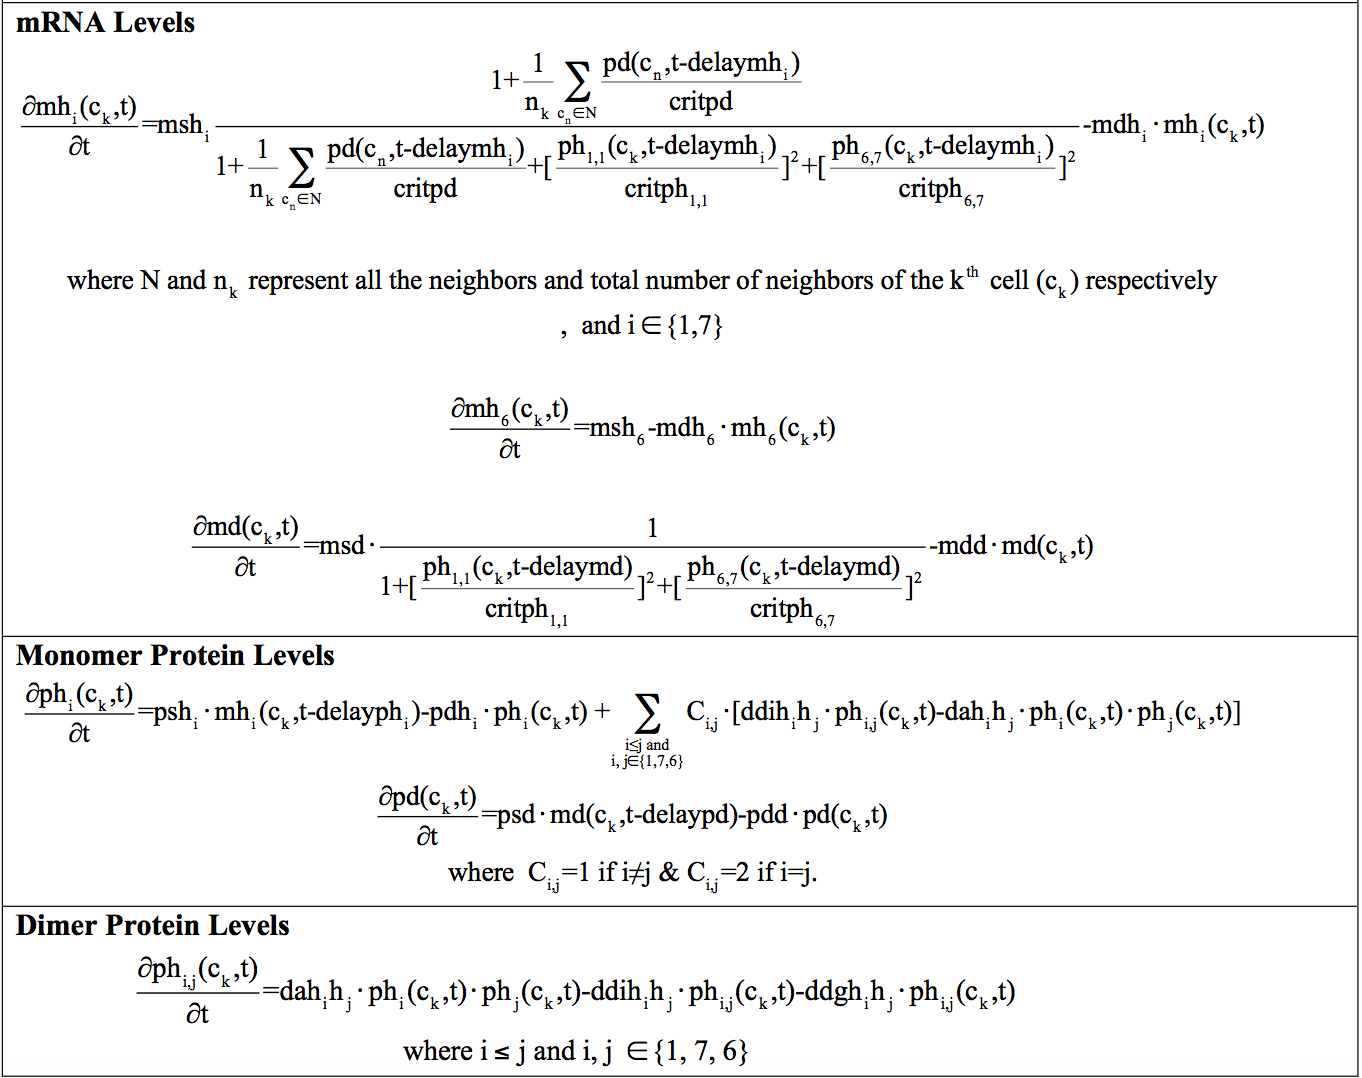
\includegraphics[width=0.9\textwidth]{3}
\caption{Differential Equation for One Reaction}
\label{fig:step3}
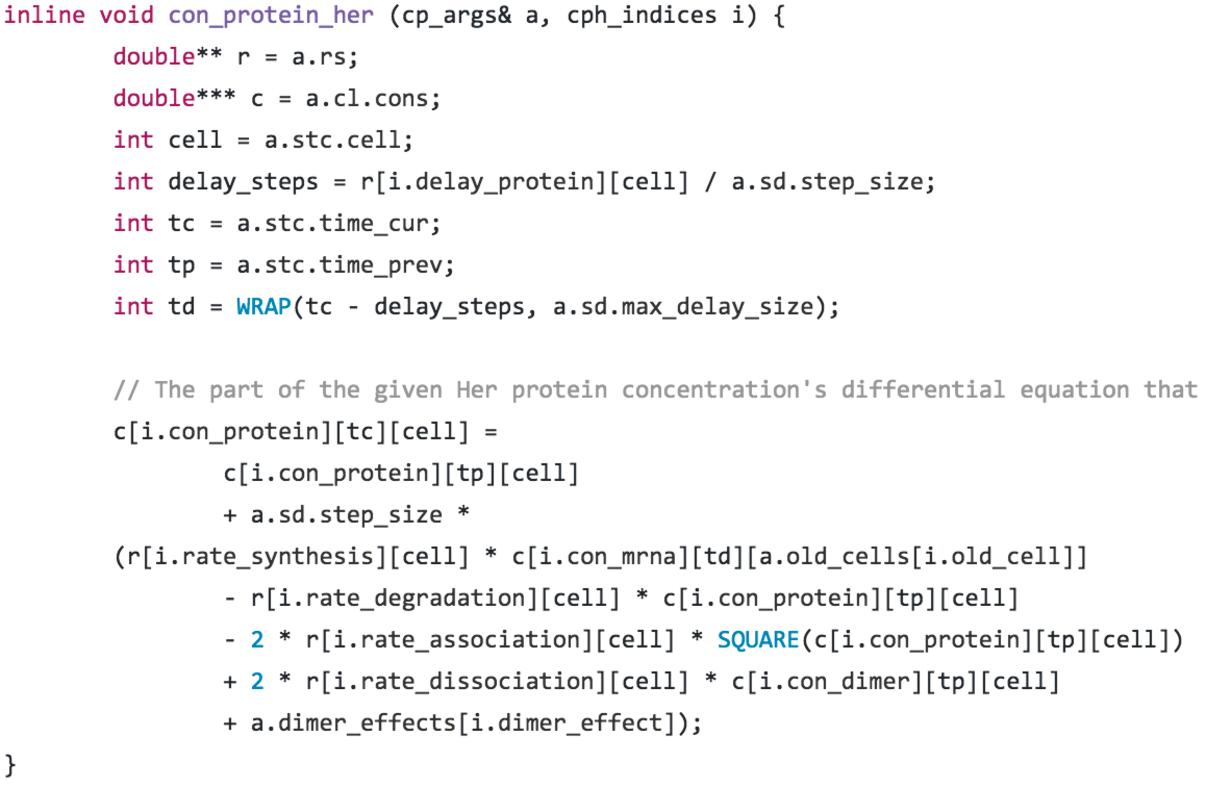
\includegraphics[width=0.9\textwidth]{oldeuler}
\caption{Implementation of \textit{Euler's Method} for Rection}
\label{fig:oldeuler}
\end{figure}
\end{document}
